\section{Layer~6 – Meta‑Learning (Learning How to Learn)}
\label{sec:layer6}

% ----- SUPERKRACHT -----
\begin{tcolorbox}[colback=blue!5, colframe=blue!60, title=\textbf{Superpower: The Meta‑Learner}]
\begin{center}
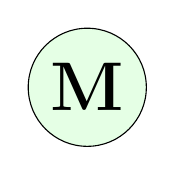
\begin{tikzpicture}
  \node[draw, circle, fill=green!10, minimum size=1.5cm, font=\bfseries\Huge] {M};
\end{tikzpicture}
\textit{“Can I learn to learn faster?”}
\end{center}
\end{tcolorbox}

Pixel is already a fast learner, but he asks himself: \emph{can I
improve the act of learning itself?}  Layer~6 looks not at what Pixel
learns, but at \textbf{how} he learns.

\begin{tcolorbox}[colback=yellow!5, colframe=yellow!80, title=Real‑life analogy]
Have you ever changed your study method?  At first you just read the
text, but later you discovered you remember far more by making
summaries or explaining the material to a friend.  You learned
\emph{how to learn}.  That is exactly the leap Pixel makes now.
\end{tcolorbox}

\textbf{Pixel’s meta‑trick.}
Pixel tries out different ways of adjusting its parameters – sometimes
with small steps, sometimes with larger leaps, sometimes with a memory
of previous adjustments.  It keeps track of which strategy yields the
fastest results and switches to it automatically.  Eventually Pixel
possesses a personal collection of \textbf{learning strategies} that
it can deploy whenever it encounters something new.

This is the reason human babies learn so fast: they are programmed to
learn how to learn.  Pixel now gets that gift too.